% This is "sig-alternate.tex" V1.9 April 2009
% This file should be compiled with V2.4 of "sig-alternate.cls" April 2009
%
% This example file demonstrates the use of the 'sig-alternate.cls'
% V2.4 LaTeX2e document class file. It is for those submitting
% articles to ACM Conference Proceedings WHO DO NOT WISH TO
% STRICTLY ADHERE TO THE SIGS (PUBS-BOARD-ENDORSED) STYLE.
% The 'sig-alternate.cls' file will produce a similar-looking,
% albeit, 'tighter' paper resulting in, invariably, fewer pages.
%
% ----------------------------------------------------------------------------------------------------------------
% This .tex file (and associated .cls V2.4) produces:
%       1) The Permission Statement
%       2) The Conference (location) Info information
%       3) The Copyright Line with ACM data
%       4) NO page numbers
%
% as against the acm_proc_article-sp.cls file which
% DOES NOT produce 1) thru' 3) above.
%
% Using 'sig-alternate.cls' you have control, however, from within
% the source .tex file, over both the CopyrightYear
% (defaulted to 200X) and the ACM Copyright Data
% (defaulted to X-XXXXX-XX-X/XX/XX).
% e.g.
% \CopyrightYear{2007} will cause 2007 to appear in the copyright line.
% \crdata{0-12345-67-8/90/12} will cause 0-12345-67-8/90/12 to appear in the copyright line.
%
% ---------------------------------------------------------------------------------------------------------------
% This .tex source is an example which *does* use
% the .bib file (from which the .bbl file % is produced).
% REMEMBER HOWEVER: After having produced the .bbl file,
% and prior to final submission, you *NEED* to 'insert'
% your .bbl file into your source .tex file so as to provide
% ONE 'self-contained' source file.
%
% ================= IF YOU HAVE QUESTIONS =======================
% Questions regarding the SIGS styles, SIGS policies and
% procedures, Conferences etc. should be sent to
% Adrienne Griscti (griscti@acm.org)
%
% Technical questions _only_ to
% Gerald Murray (murray@hq.acm.org)
% ===============================================================
%
% For tracking purposes - this is V1.9 - April 2009

\documentclass{sig-alternate}
\usepackage{color}

%%%% User-defined macros
\newcommand{\lam}{\lambda}
\newcommand{\mycomment}[1]{\textcolor{red}{#1}}
%%%%% Uncomment this line (and comment the previous one)
%%%%% to remove all comments
%%%%% NOTE: comments still occupy a line even if invisible;
%%%%% Don't write them as a separate paragraph
%\newcommand{\mycomment}[3]{}

\begin{document}

%
% --- Author Metadata here ---
\conferenceinfo{UMM CSci Senior Seminar Conference, April 2014}{Morris, MN}
%\CopyrightYear{2007} % Allows default copyright year (200X) to be over-ridden - IF NEED BE.
%\crdata{0-12345-67-8/90/01}  % Allows default copyright data (0-89791-88-6/97/05) to be over-ridden - IF NEED BE.==
% --- End of Author Metadata ---

\title{
Applying Evolutionary Computation to Robotics}
%\subtitle{[Extended Abstract]
%
% You need the command \numberofauthors to handle the 'placement
% and alignment' of the authors beneath the title.
%
% For aesthetic reasons, we recommend 'three authors at a time'
% i.e. three 'name/affiliation blocks' be placed beneath the title.
%
% NOTE: You are NOT restricted in how many 'rows' of
% "name/affiliations" may appear. We just ask that you restrict
% the number of 'columns' to three.
%
% Because of the available 'opening page real-estate'
% we ask you to refrain from ElenaSampleputting more than six authors
% (two rows with three columns) beneath the article title.
% More than six makes the first-page appear very cluttered indeed.
%
% Use the \alignauthor commands to handle the names
% and affiliations for an 'aesthetic maximum' of six authors.
% Add names, affiliations, addresses for
% the seventh etc. author(s) as the argument for the
% \additionalauthors command.
% These 'additional authors' will be output/set for you
% without further effort on your part as the last section in
% the body of your article BEFORE References or any Appendices.

\numberofauthors{1} %  in this sample file, there are a *total*
% of EIGHT authors. SIX appear on the 'first-page' (for formatting
% reasons) and the remaining two appear in the \additionalauthors section.
%
\author{
% You can go ahead and credit any number of authors here,
% e.g. one 'row of three' or two rows (consisting of one row of three
% and a second row of one, two or three).
%
% The command \alignauthor (no curly braces needed) should
% precede each author name, affiliation/snail-mail address and
% e-mail address. Additionally, tag each line of
% affiliation/address with \affaddr, and tag the
% e-mail address with \email.
%
% 1st. author
\alignauthor
Adrian T. Schiller \\
\affaddr{University of Minnesota, Morris} \\
\email{schil227@morris.umn.edu}
}

\maketitle
\begin{abstract}

\end{abstract}

%% A category with the (minimum) three required fields
%\category{H.4}{Information Systems Applications}{Miscellaneous}
%%A category including the fourth, optional field follows...
%\category{D.2.8}{Software Engineering}{Metrics}[complexity measures, performance measures]

%\terms{Evolutionary Computation, Robotics, Simulation, Neural Networks, Evolutionary Robotics}

\keywords{Evolutionary Robotics, Evolutionary Computation, Robotics, Neural Networks, Evolved Behaviors, Locomotion, Simulation}


%	The limitation of only being able to evolve small parts of programs is an issue in evolutionary computation (EC) \mycomment{am I BS'ing or is this legit?}. Much of these constraints are due to there is no graceful way to evolve programs, as a whole, directly at the source code. This is because source code exists to make it easier for humans to read and write code. However, it is very hard to create a genetic algorithm (GA) that would evolve source code. Even if one was created it would basically be the size of a compiler \mycomment{Need to review the compiler argument in finch. feel like I'm BS'ing}.
%	A solution to this problem is to to compile the program into a lower level language and evolve it there. Two lower level languages at which this has been done is Java bytecode and x86 assembly~\cite{FINCH:2010}~\cite{Assembly:2010} which I will discuss thoroughly in this paper ~\mycomment{add more}.
	
\section{Introduction}
 As robots become increasingly automated, they are subject to more environments and actions. The problem with these scenarios is that it requires more complex development to account for the numerous cases that a robot may encounter. Evolutionary Computation (EC) is a very useful tool for solving complex problems, and applying EC to robots seems ideal for developing complex behaviors.
 
 However, EC requires intensive computation for hours at a time, generating, modifying, and evaluating many candidates. This becomes impractical for a physical robot because it would require the overhead of uploading the code, setting up the robot to be identical every time it is tested, running the robot in the exact same environment, and doing each of these task  thousands of times. EC for robotics is especially infeasible because it is done in real time, as opposed to traditional EC. Because of the percision and time required, it is unclear how to make EC effective in robotics.
 
 Yet means do exist to apply evolution to robotics, an area known as Evolutionary Robotics (ER). The purpose of this paper is to analyze what methods are used to create the evolutionary process for physical machines, the effectiveness of their outcomes, and the general feasibility of ER.
 
 This paper will analyze three different research cases involving evolutionary robotics. By noting their similarities and differences, some idea can be generated of what ER requires. The research outcomes will demonstrate the effectiveness of the evolutionary process.

   Section \ref{background}  has  background information on evolutionary computation, neural networks, and the research cases this paper uses. Section \ref{simulation} covers robotic simulation and how it's used in the research cases, section \ref{evolution} gives the details about the evolutionary robotics for each of the research cases, and section \ref{behavior} discusses behaviors the evolved robots developed, and section \ref{conclusion} is the conclusion.
 
 
%\section{The {\secit Body} of The Paper}\label{main}
\section{Background}\label{background}
In order to understand the complexities behind evolution and robotics, we must define the evolutionary computation, genetic algorithms, and neural networks, Three research cases will be introduced as well.

 \subsection{Evolutionary Computation}\label{background EC}
  Evolutionary computation (EC) is described by Sipper ~\cite{Sipper2011Win} as solving a problem by tweaking a population of candidates and evaluating them by some quantifiable fitness. This process then repeats until a suitable candidate can be found or a set limit is reached (e.g. time). The concept can be compared to natural genetics and evolution.
  
  Genetic Algorithms (GA) \cite{wiki:GeneticAlgorithms}, a type of EC, mimics natural selection by using a population of candidates whose success is quantified by a fitness function, and then used to create the next generation of individuals. When populating the next generation, candidates are commonly crossed-over with one another, which produces two new individuals based on the candidates. Mutation is another means of modifying a candidate, which is the random chance  of slightly changing the candidate. The cross-over/mutation process repeats until the new population is created. This process  repeats until a suitable candidate can be found or a limit is met.
  
  A sample problem which GA can be applied to is ``One Max": Suppose there is a population of $p$ candidates which are arrays of length $n$ whose elements are randomly set either zero or one, and the goal is to evolve a candidate array that consists of entirely ones. In the first iteration, the fitness function would be applied which would return the number of ones in an array, and then sort the population of candidates from greatest fitness to least. Then, some subset of the population, $m$, is chosen to populate the next array of candidates ($m$ for example, could contain the 20 best individuals). The $m$ candidates that move on would then be used to create the next generation of candidate arrays via cross-over/mutation until $p$ candidates are constructed. In this example, the crossover process takes two fit candidate arrays and swap parts from either array to make two new candidate arrays. These candidates may also undergo some mutated, such as swapping a random bit in the array. This process then continues until a suitable candidate is reached, or a time/iteration limit is reached. The result is the candidate with the highest fitness; in this example the candidate with the most ones.
  
\subsection{Neural Networks}
	A Neural Network (NN) \cite{wiki:robotics} is an algorithm which is based loosely on the central nervous system in biology. In EC, a NN is referred to as an Artificial Neural Network (ANN) to distinguish between a physical neural network and those artificially generated in programs. The network is a collection of nodes (``neurons") which are connected in a network. The network is composed of several weighted verities (synapses in the biology analogy) between all the nodes in the network, and act as a control structure to alter the input as it is passed to the output. The purpose of the network is to develop an approximated relationship between a given input and a desired output.

	 The ANN has three general layers: input, middle, and output. The input layer is composed of whatever input is provided; in the case of a robot, it could be motor controllers and other sensors. Each sensor or motor would be a separate node. The middle layer is the hidden layer where the evolutionary process occurs. From the genetic algorithm example in \ref{background EC}, instead of swapping bits in an array, weights of the network would be swapped or altered. The middle layer is not necessarily only one layer, but for the purposes of this paper it is considered a single layer. The output layer is the result of the weighted inputs. For example, there could be an ANN which takes in the velocity of a car and how long it has driven as it's input, and the output could be a coordinate on the $xy$-plane of it's location, calculated from a mathematical formula developed in the hidden layer. Figure \ref{fig:ANN} is an example of an ANN. Two of the three research cases presented in this paper use neural networks (\cite{Moore:2013:ESK:2463372.2463402},~\cite{Pretorius:2009:TAN:1632149.1632171}).
  
  
  \subsection{Research Cases}
	This paper compares and contrasts three separate research cases which used Evolutionary Robotics. Each research study used three common approaches to apply evolution to find a solution for a physical robot; a simulation, an evolutionary process, and behavioral analysis of evolved candidates.
	
	The first study, done by Moore $et$ $al.$~\cite{Moore:2013:ESK:2463372.2463402}, is a simple floating aquatic robot which is tasked with maintaining a particular position while being subject to water flowing in a common direction, also known as laminar flows. The robot has a cylindrical body with three servo controlled fins; two flippers which have 360$^\circ$ of circular movement range and a caudal (rear) fin which has 30$^\circ$ of movement. Figure \ref{fig:sRobot} shows the robot in simulated and physical form. The robot is equipped with an inertial measurement unit (IMU) which measures linear and angular acceleration, and is able to provide a 3D coordinate of the robot's current position. ER was chosen for finding a solution because of the variety of directions the robot could encounter laminar flows.

\begin{figure*}%[H]
\center
  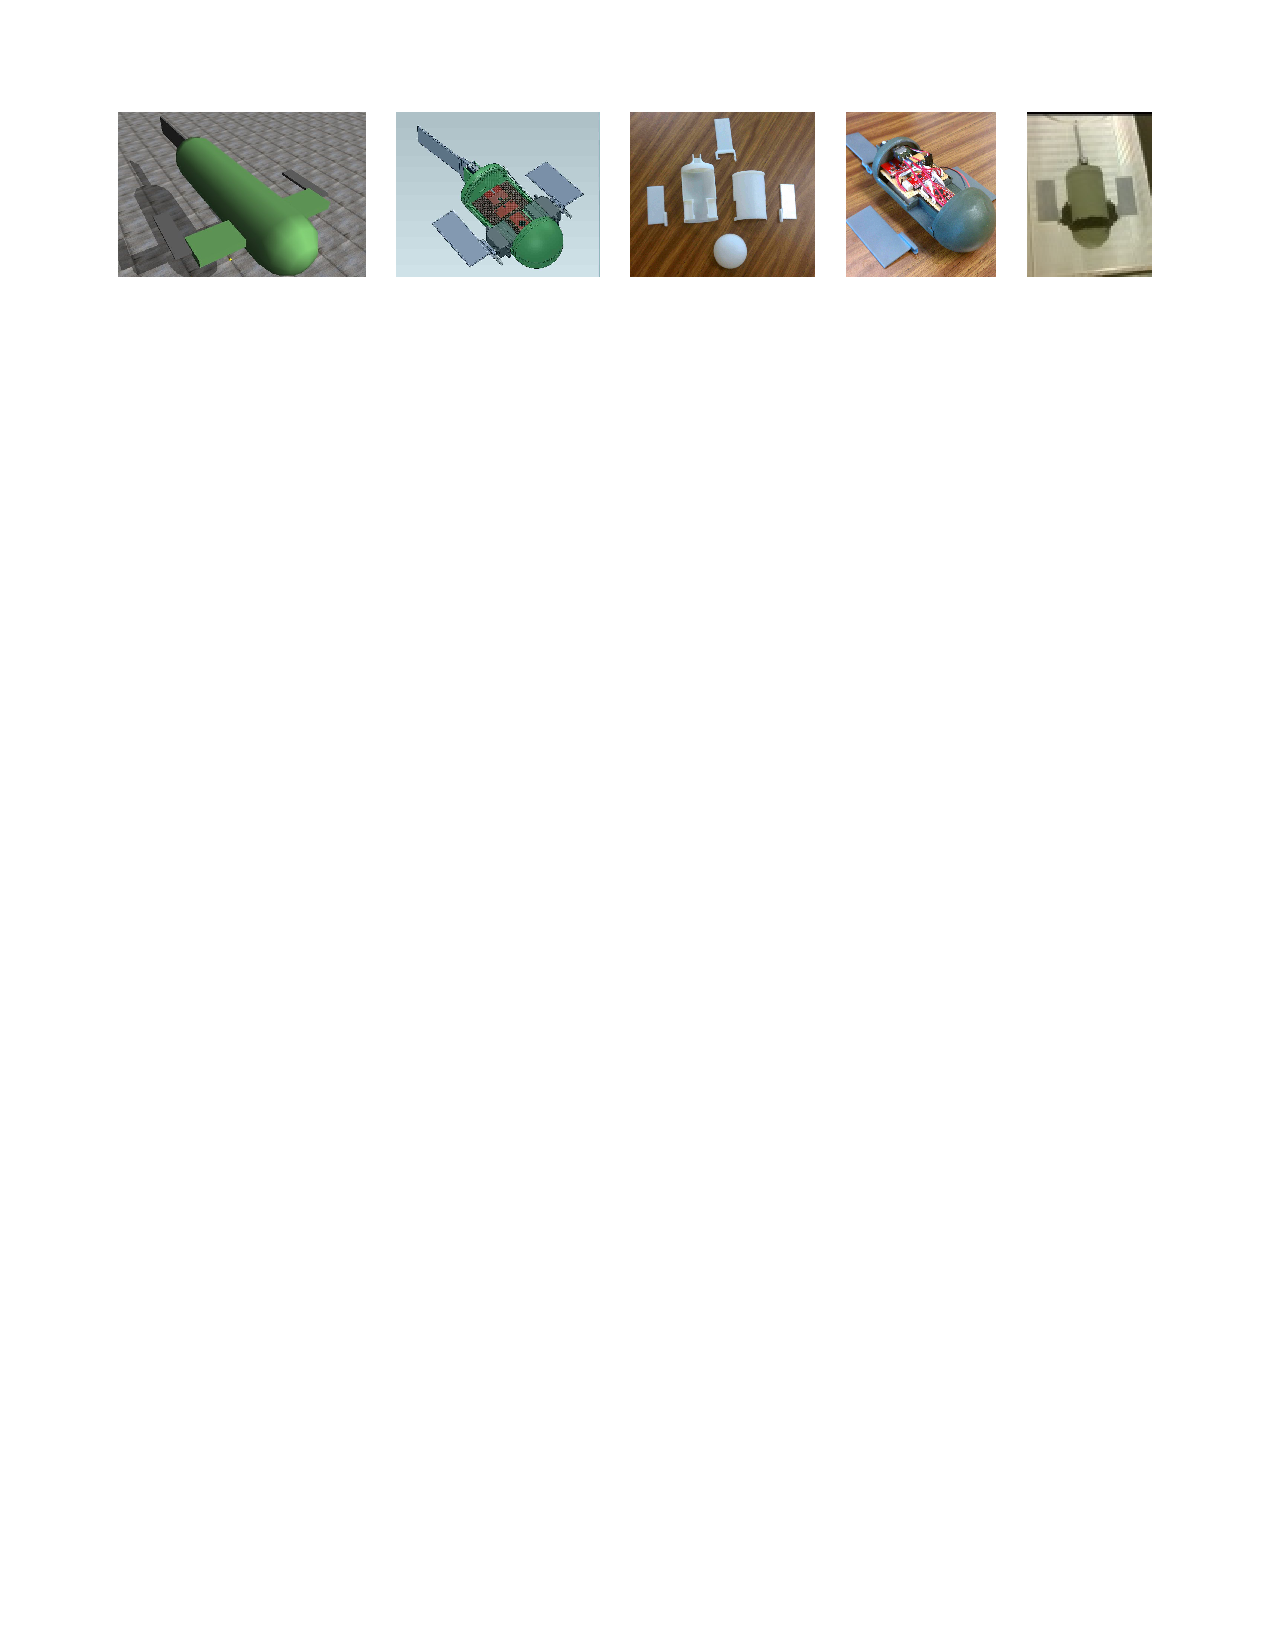
\includegraphics[scale=1]{sr2}
\caption{The station keeping robot rendered in simulation as well as it's physical form}
\label{fig:sRobot}
\end{figure*}

	
	The next study, conducted by Farchy $et$ $al.$ ~\cite{Farchy:2013:HRL:2484920.2484930}, was to increase the walking speed of a humanoid robot. The robot model known as the Aldebaran Nao (Figure \ref{fig:wRobot}), is programmed by teams to play (robot) soccer in a competition called RoboCup. The process by which  Farchy $et$ $al.$ applied ER was through Grounded Simulation Learning (GSL), which added human guidance to the evolutionary process (more on GSL in section \ref{Farchy Evolving}). 
	
\begin{figure}%[H]
\begin{center}
  \includegraphics[scale=1]{wr1}
\end{center}
\caption{The Aldebaran Nao Robot, programmed to play soccor}
\label{fig:wRobot}
\end{figure}

	The final study, by Pretorius $et$ $al.$ ~\cite{Pretorius:2009:TAN:1632149.1632171}, created a Lego Mindstorm robot which would track its own position and heading from an evolved controller. This controller would be able to calculate where the robot is located as it moves,while only using the motor's speed, direction, and running time. The robot (Figure \ref{fig:pRobot}) consists of two motorized wheels and has two blue and purple tracking markers on the top, as well as a light sensor. The markers and light sensor were used by an overhead camera to collect position and orientation information, and pair it with commands given to the robot. This data was used as a testbed to train the controller. This is a difficult problem because without sensory input, tracking a position must be done using internal functions, which tend to be complex because of various acceleration the robot undergoes when moving. ER was chosen to create a correlation between motor movement and location/orientation. 

\begin{figure}%[H]
  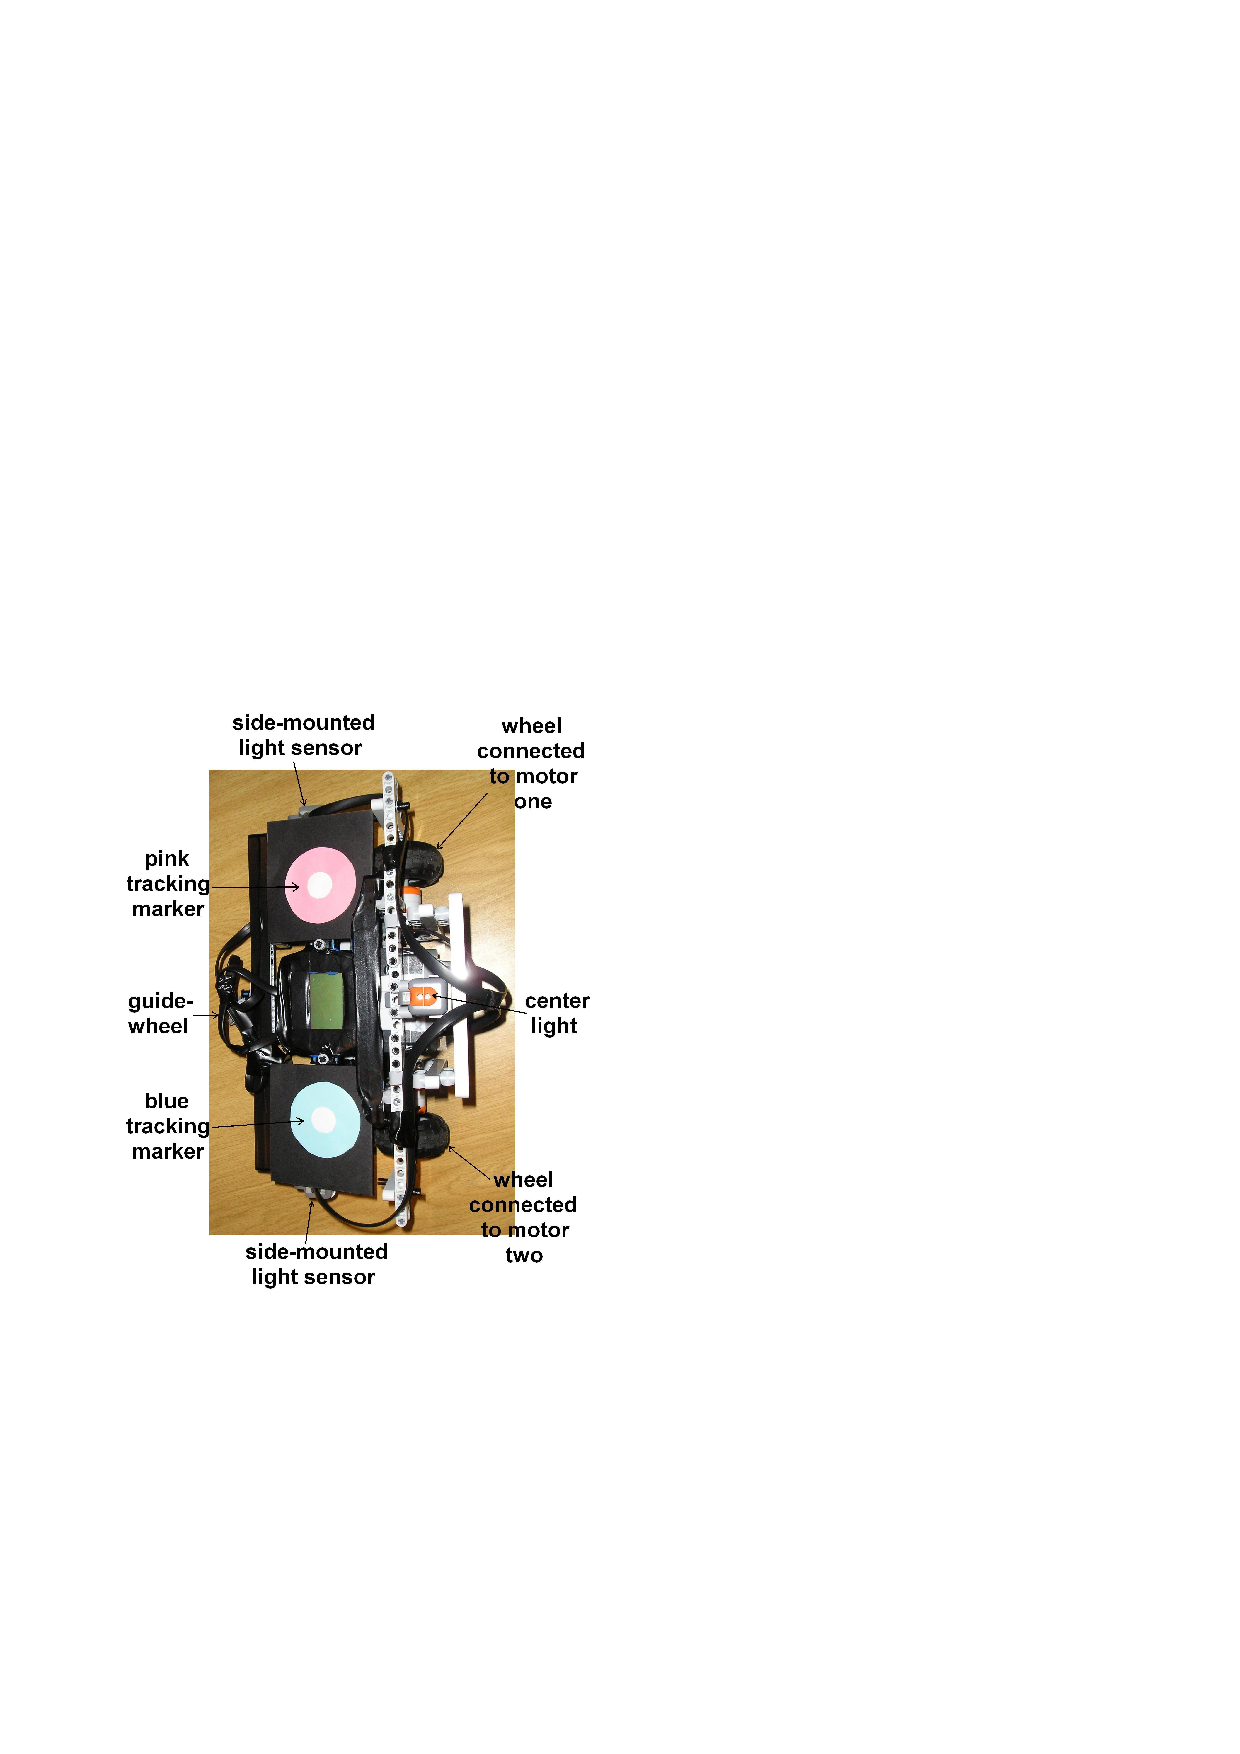
\includegraphics[scale=1]{cr1}
\caption{The position tracking robot}
\label{fig:pRobot}
\end{figure}
	
\section{Simulation}\label{simulation}
Evolution in robotics is expensive because of the overhead of running trials in real time and setting up the robot to be identical for each test. Simulation is valuable because it can explore the space of ER at an accelerated rate without requiring setup. Simulation is the representation of characteristics or behaviors of one system through the use of another system. Simulation provides a means through which a replica  of the robot can be rapidly altered and evaluated, thereby enabling the evolutionary process to occur. However, because simulations are often imperfect representations of the physical space, there is some measure of error by transitivity.

Transitivity in this case is defined as inaccuracies between the simulated and physical robot and the simulated/physical environment ~\cite{Farchy:2013:HRL:2484920.2484930}. Small inaccuracies can sometimes lead to poor performance; that is, when a candidate performs well in simulation, but performs poorly with the physical robot. For example, if a simulation had assumed the surface a walking robot was moving on was a completely level plane, but in actuality it was slightly sloped; we could envision a robot which evolved to perform well in the simulation but might be unable to handle the change in slope and perhaps fall down. Therefore it is critical to have a simulation which has little transitivity error when applying ER.

 Moore $et$ $al.$  ~\cite{Moore:2013:ESK:2463372.2463402}evolved floating station keeping robots with a simulator which uses the Open Dynamics Engine (ODE). The simulated environment updated every 5 ms to calculate the next state of the robot and environment. It provides a system to calculate forces applied to the simulated robot in a body of water, but does not have fluid dynamics. Instead, physical drag is applied to each of the faces of the simulated robot. Propulsion is found to be the net force generated by each of the faces against the drag, which determine the next state of the robot. Fluid dynamics are computationally intensive and require a lot of processing to do accurately. Alternatively, creating a simple model requires much less CPU processing time and therefore scales better for evolving candidates. Moore $et$ $al.$ noted that an extremely accurate simulation was not a priority because they were more interested in the evolved behaviors, that is solutions the evolved candidates create, rather than exact specifications (See Behavioral Analysis \ref{Moore behavior}).
 
 The robot walking code modified by Farchy $et$ $al.$~\cite{Farchy:2013:HRL:2484920.2484930} used SimSpark, a simulation based on the RoboCup tournament which also uses the ODE for rigid body movement and collision detection (Figure \ref{fig:simSpark}). It is not a perfect simulation however, and lacks important features such as joint friction. Unlike the station keeping robots, transitivity errors pose more of an issue because of the threat of the physical robot being immobilized (e.g. falling over). Every 20 ms the simulator updates the state of the robot by using sensor information  fed into the simulation. The robot used in the simulator is not the same model as the physical one used by Farchy $et al$, requiring approximations of key features such as the shape of the foot. However, Farchy $et$ $al.$ employed a ``Grounded Simulation Learning'' (GSL) algorithm, which, like the station keeping robot study, was used for finding developed behaviors and, in this case, modifying the evolutionary process from the analysis. GSL also accommodates for inaccuracies in the simulation by routinely analyzing if evolved controllers are indeed applicable to the physical robot.
 
 \begin{figure}%[H]
 \begin{center}
  \includegraphics[scale=1]{wr2}
 \end{center}
\caption{The SimSpark simulation}
\label{fig:simSpark}
\end{figure}
 
 The simulation used by Pretorius et. al.~\cite{Pretorius:2009:TAN:1632149.1632171} used a more unorthodox method. As opposed to using a physical simulator (such as ODE), they chose to use artificial neural networks as the simulator. The reason the team went with this option is because a physics engine, as previously stated, contains minute inaccuracies which can affect the results. In this case, the simulator is also what is being evolved, the goal being to create a simple navigation controller which would effectively simulate the robot's location and direction. By driving the robot over a surface using arbitrary motor commands, and tracking the position and orientation with an overhead camera, they were able to extract data to be used as a testbed for the evolutionary process. In this case, the error caused by transitivity is relative to how accurately the camera captured the position and orientation of the robot. Fortunately, the relative error was fairly small because the captured results were within 2 cm of the physical robot's position. 
 
 In each of the research cases, there was a way in which the process of evaluating the robot was taken from the physical condition and placed in simulation. The simulation then enabled evolutionary robotics to avoid the overhead of physical testing and to happen at an accelerated rate. By transferring the actions of the robot and the physical environment into a simulation, it allows ER to be feasible done in a reasonable amount of time.

\section{Neural Network, Experiment, and Evolving Process}\label{evolution}
  The process of evolving candidates (addressed in section \ref{background}) was applied to each of the research robots. This section details how each case applied ER, including population size, number of generations, how they implemented neural networks, fitness functions and evaluation methods.
  \subsection{Station Keeping Robot}\label{Moore Evolving}
  The input of the ANN for the station keeping robot ~\cite{Moore:2013:ESK:2463372.2463402} was the current position of the robot in three dimensional coordinates, $(x,y,z)$, the difference between the the robot's current position and the desired position, and the previous output. The output nodes were the oscillation of the Caudal fin, and speed of the flipper servos. The desired outcome of this neural network is to have the robot properly orient itself and maintain a fixed position based on the input.
  
 The simulated robot was subjected to 4 different types of Laminar flows; from the front, the back, the side (90$^\circ$ from the front), and at a 45$^\circ$ angle from the front left. Because Moore $et$ $al.$~\cite{Moore:2013:ESK:2463372.2463402} was interested in behaviors evolved by the robot, each of these trials was a separate evolutionary process so as to not create a single candidate which had to perform well in all four. A transient period was used, which allotted 60 seconds for the robot to adjust to the particular flow. This was because early candidates would try to immediately maintain the position and have poor results; the transient period allowed the candidate to reorient itself to better maintain the position without an early penalty. 
 
 The evolutionary process used a population of 100 candidates and evolved them for 2000 generations. Each of the four trials replicated the evolutionary process 25 times. After the 60 second adjustment phase, the simulated robot candidate was evaluated every 250 ms for the next 60 seconds. The robot's total fitness was the summation of the evaluated fitness every 250 ms;

\begin{equation*}
	\textrm{fitness} = \sum_{t} (10 - d_t(x, y, z))
\end{equation*}
where
\[
	d_t(x, y, z) = 
		\begin{cases} 10, & \textrm{if distance}_t(x, y, z) > 10 \\
					  \textrm{distance}_t(x, y, z), & \textrm{ otherwise}
		\end{cases}
\]
 
 
  where the distance function is how far the robot's position was from the desired location. The $10$ in the fitness function is an arbitrary number to quantify the fitness of the candidate. The fitness is modified to have a gradient effect when the robot is close to the target location, which incentivizes continual station keeping.  
 
  \subsection{Walking Humanoid Robot}\label{Farchy Evolving}
  The walking robot  ~\cite{Farchy:2013:HRL:2484920.2484930} had 17 different parameters, including \texttt{stepPeriod}, $\texttt{amp}_\texttt{swing}$, \texttt{startLength}, etc. which essentially act as functions that alter multiple joints in the robot walk cycle. Farchy $et$ $al.$ applied ER to optimize the parameters to increase the standard walking speed. It is worth noting that they didnt use an ANN, and instead evolved the parameter sets with different values using a GA-like algorithm.
 
 The robot was evaluated in two separate trials. The first trial, {\tt goToTarget}, gave the simulated robot several locations to walk to, dealing with several changes in direction. The fitness of {\tt goToTarget} is:
\[
  \textrm{fitness} = \sum_{t} (\textrm{DistanceTraveled}_t) - \textrm{fallingPenalty}
\] 

 where {\tt DistanceTraveled} is the the length between each destination. All of the {\tt DistanceTraveled} values are summed until the trial ends or the robot falls down. {\tt FallingPenalty} is a penalty administered to the fitness should the robot fall before completing the trial, and is not included in the summation. The other trial is {\tt WalkFront}, which evaluates the velocity of the robot walking forward for 15 seconds. The robots fitness for {\tt WalkFront} is the maximum velocity it achieves. Together, these two trials evaluate how quickly a robot can move and how stable it is, evolving a both fast and stable robot.
  
  Farchy $et$ $al.$ used an algorithm slightly different from GA called Co-variance Matrix Adaptation Evolution Strategy (CMA-ES). The main difference between the two is CMA-ES tracks a co-variance matrix of parameters which perform well, thereby drawing a correlation between well performing candidates and their parameters. Instead of sorting solely by fitness like GA, it sorts by these parameters and repopulates the next generation by the upper mean of the previous generation.
  
  One of the most interesting consepts done by Farchy $et$ $al.$ ~\cite{Farchy:2013:HRL:2484920.2484930} and the focus of their research was the use of Grounded Simulation Learning (GSL). GSLis composed of two main parts: grounding and guidance. Grounding refers to making the simulation's behavior match the physical robots behavior; this reduces problems with transitivity. Guidance refers to human interaction in the simulation to make strategic adjustments in the evolutionary process. GSL was applied after each iteration to focus on evolving specific features, such as taking longer strides or improving better. For example, after the first iteration of evolution the team uploaded the candidate to the physical robot and noticed that the leg swing parameter seemed to play an important role in the speed of the robot. The next iteration was then adjusted to have greater variation in the swing parameter to be used in the CMA-ES algorithm. 

  \subsection{Position Tracking Robot}\label{Pretorius Evolving}`
  To train the position tracking robot's ANN, the robot was issued commands ~\cite{Pretorius:2009:TAN:1632149.1632171}  consisting of three things: motor speeds and the directions of each of the motors, and the execution time for the command in milliseconds. The motor speed was randomly generated which ranged up to 50\% of it's maximum, and the time ranging from .5 to 3 seconds. Although random, there was bias to have the motors go in the same direction at an equal speed (straight movement) 30\% of the time, as well as both motor speeds to equal 0 (stopping the robot) 20\% of the time. This was because  Pretorius $et$ $al.$ felt that these would be common commands, and should be represented well in the simulation.
  
  Pretorius $et$ $al.$ used three different simple ANNs to track the robot's position. Similar to how the station keeping robot evolved four different candidates for each of the laminar flows, using three different networks removed the demand for a single network to perform well in tracking both coordinates and the orientation. The input to each of the neural networks consisted of the two motor speeds before receiving the command, the two motor speeds from the current command, and the length of time for the current command. The purpose of using the previous motor command was to account for positive and negative acceleration the robot underwent going from one command to the next; the neural network would have to incorporate that change in order to make an accurate account of it's orientation. The output of each of the ANNs was either the robot's x-coordinate, y-coordinate, or angle. Figure \ref{fig:ANN} is a visual representation of the ANNs.
  
\begin{figure}%[H]
\begin{center}
  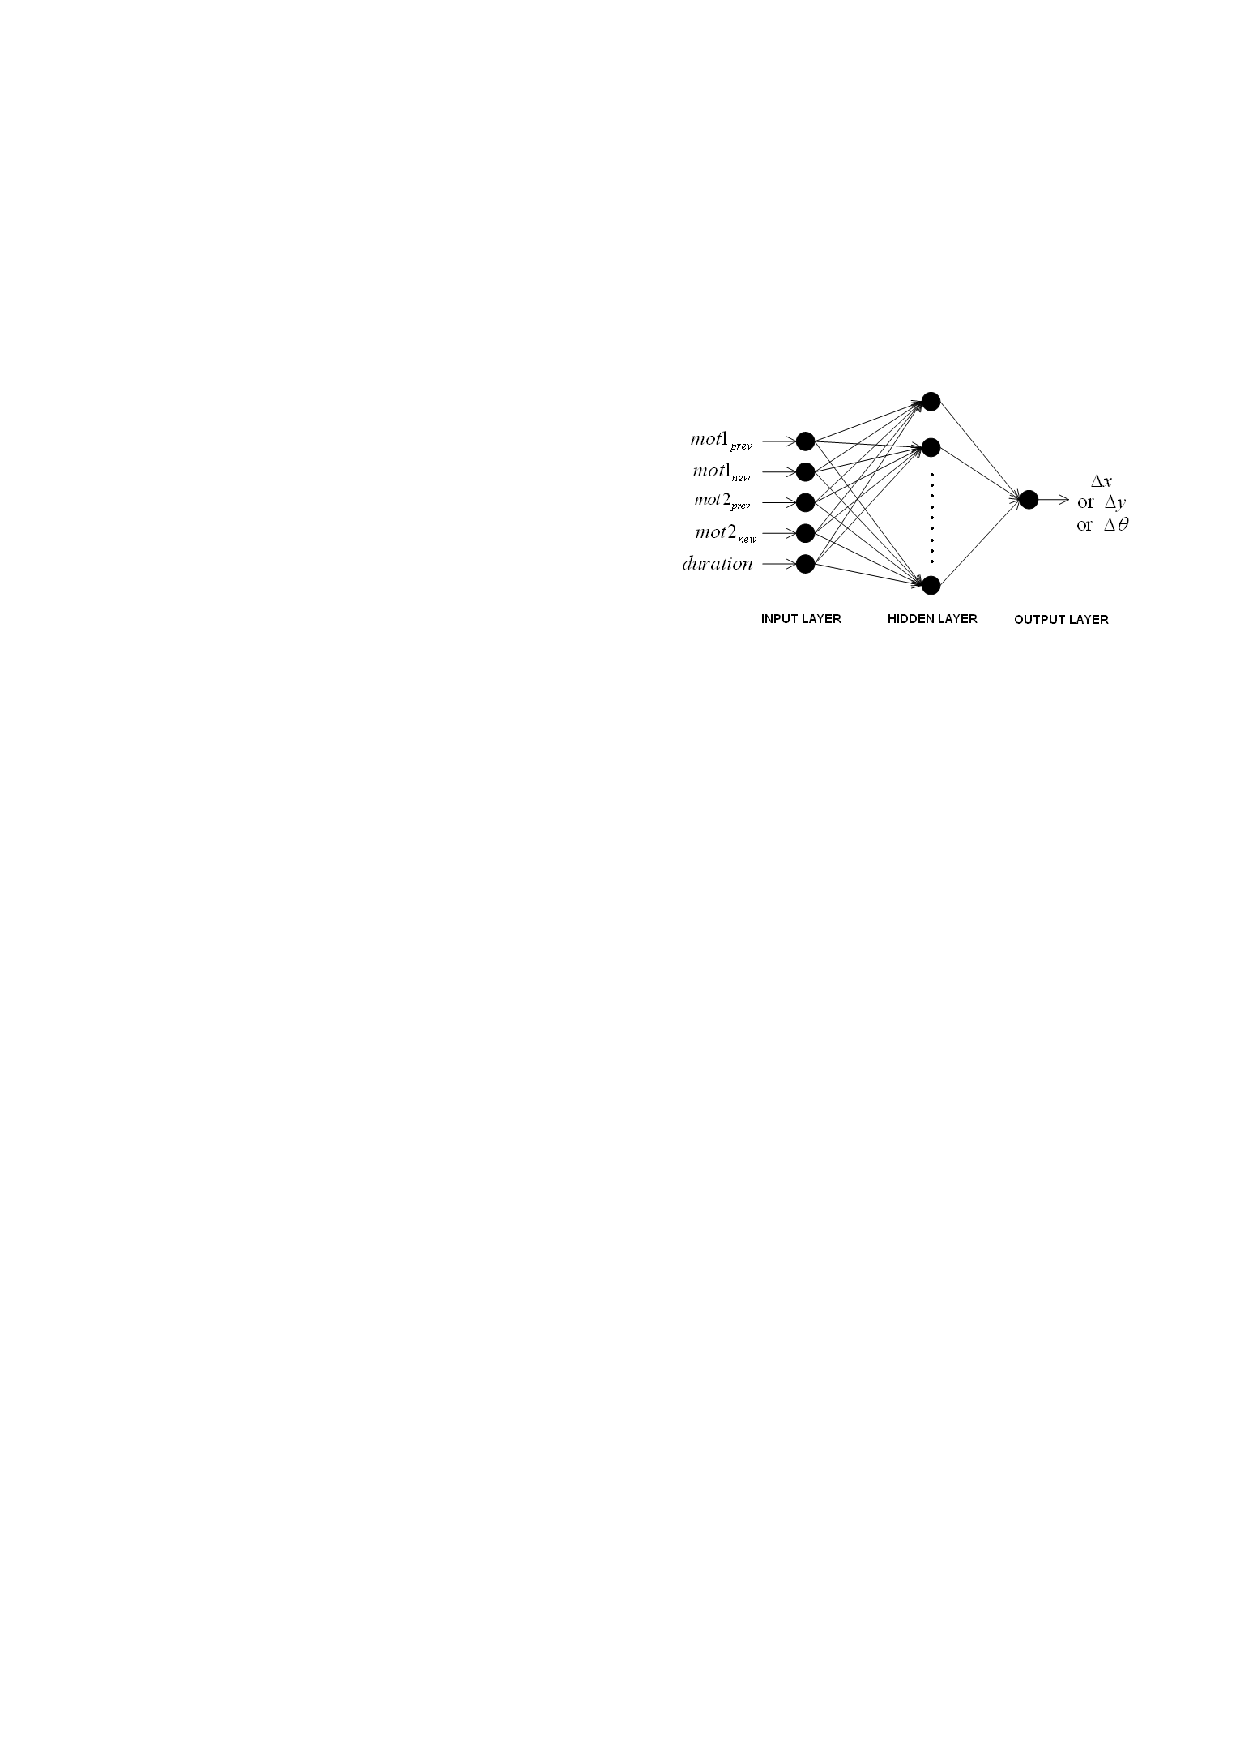
\includegraphics[scale=1]{cr2}

\end{center}
\caption{The ANN for the position tracking controller}
\label{fig:ANN}
\end{figure}

  The ANNs were then evolved using a GA. The GA parameters included a 80\% crossover probability and a 5\% mutation possibility. The population size was 250 candidates, which were evolved for 15,000 generations. This took approximately 12 hours for each of the three ANNs. The fitness function was the Mean Squared Error (MSE), which measured the accuracy of a given candidate ANN configuration. The MSE is defined as:
  
  \[
  \textrm{fitness} = \frac{1}{N}\sum\limits_{p=1}^N\sum\limits_{i=1}^O (t_{pi} - a_{pi})^2
\] 

  Where $N$ is the size of the testbed (i.e. the collected data from arbitrary motor commands and their physical position, as gathered from the overhead camera), $O$ is the number of outputs from the ANN, $t$ is the expected output, and $a$ is the actual output. Both $t$ and $a$ are are subject to some particular test $p$ in the testbed and for either the x-coordinate, y-coordinate, or angle, $i$.
  
  In addition to evolving the ANN controllers, Pretorius $et$ $al.$ evolved a  navigational controller, which was a set of commands, to drive the robot around a 3 by 3 rectangular grid using the evolved ANNs. The objective was to have the robot start in the center left spot and drive counter clockwise around the grid to end back up in the starting spot, while avoiding the middle rectangle, staying on the grid, and visiting each space in a procedural manner. If the navigation controller violated any of those requirements, it would be heavily penalized. The fitness function was:


\[
  \textrm{fitness} = N_{max}^2 - \frac{C_{nogain}}{10}
\] 

Where $N_{max}$ is the absolute number of rectangles traversed while not entering forbidden areas and $C_{nogain}$ is the number of commands which did not cause the robot to advance to the next rectangle.

	In order to effectively evolve the navigation controller candidates, cross-over/mutation was modified to swap parts that were relatively close to the same part in the grid which the robot would navigate. For example when crossing two candidates, the part of their structure which issued a `turn' command at the top left square of the grid would be marked as the swap point. This resulted in more consistent candidates and more effective evolution. 
\section{Results and Behavioral Analysis}\label{behavior}

  Evolved code may be confusing or difficult to alter. By observing evolved behaviors, it is possible to learn the general solution and then create code to mimic that solution. This is not a necessary step, but it can provide some insight as to what the evolved candidate is doing to be successful.

\subsection{Station Keeping Robot}\label{Moore behavior}
  The evolutionary solutions for the station keeping robot in ~\cite{Moore:2013:ESK:2463372.2463402} were both unforeseen and effective. Depending on the trial, the evolved candidates would range from standard locomotion to complex maneuvers. When the flow was coming from either the front or at a 45$^\circ$ angle to the front left, the simulated robot would swim forward or swim forward while listing to the left. Because of the design of the robot, it is somewhat difficult for it to turn and not move too far away from the starting point. This would make station keeping especially difficult when the flow was coming from the back or side, the robot would drift away as it would turn, resulting in a poor fitness. So instead, when the flow was coming from directly behind the robot, it used a complex maneuver to flip tail-over-head to face the flow and then propelled itself forward to maintain its position (http://y2u.be/UufbnEGFwV4). Figure \ref{fig:robot flip} shows the behavior. This works well because the robot floats, and the flipping movement doesn't cause a change in it's height in the water. The most challenging trial was when the flow came at a 90$^\circ$ angle; because reorienting to such an angle was a significant challenge, the evolved behavior incorporated a flipping motion combined with a rolling the body to avoid turning.
 
\begin{figure*}%[H]
\center
\caption{Images from the simulation which showed the evolved behavior when the flow was behind the robot}

  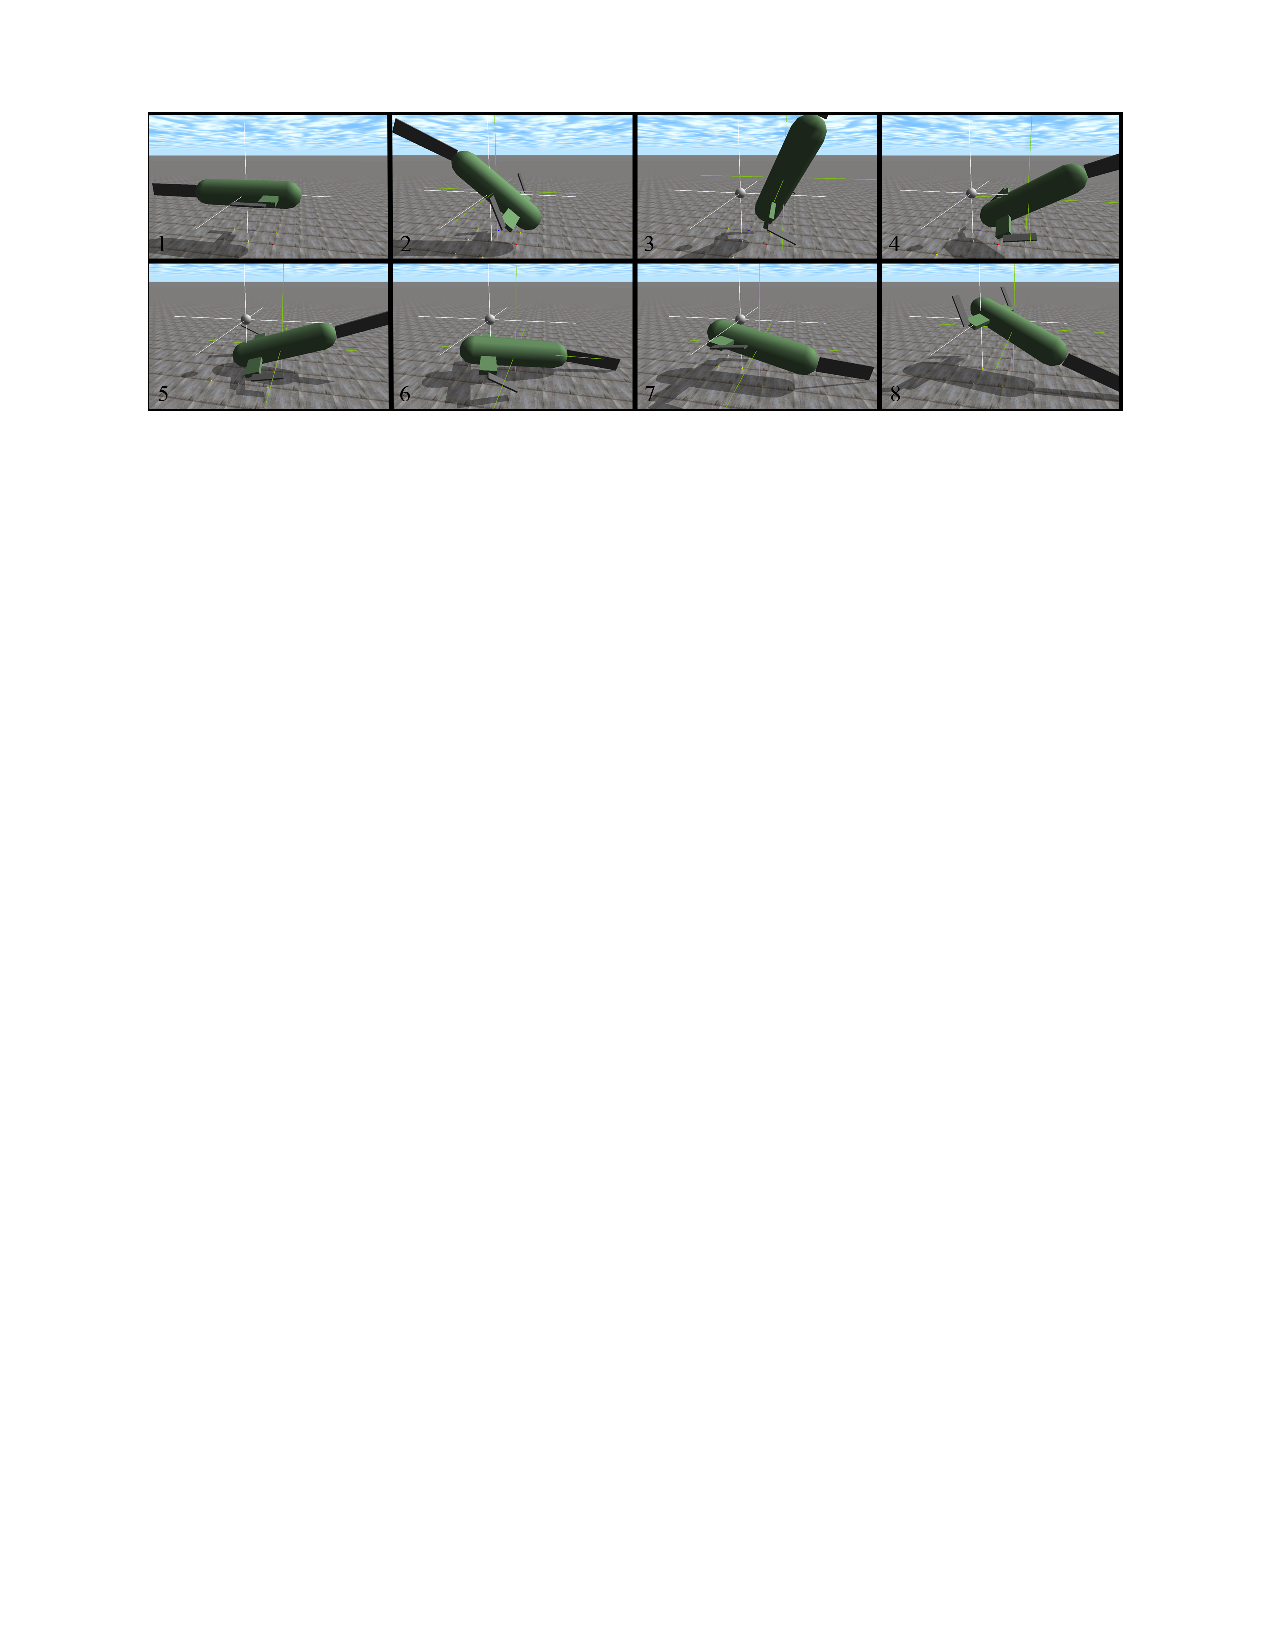
\includegraphics[scale=1]{sr1}
\label{fig:robot flip}
\end{figure*}

  Moore $et$ $al.$ compared early candidates with final candidates to contrast in evolved behaviors. When the flow was coming from behind, an early candidate selected from the 25\textsuperscript{th} generation was pushed by the current straight out of the `rewards zone' (the desired station keeping location). It didn't actually start swimming until 60 seconds into the 120 second trail, and was unable to make any progress in the allotted time. In contrast, the final candidate immediately reacts and is able to orient (flip) itself and gain against the flow into the `rewards zone'. 
% Figure \ref{rewardsZone} compares the final and an early candidate and their ability to maintain position over time.

  
  Moore $et$ $al.$ noted that one of the most impacting changes was to allow a setup phase. The setup phase allowed the candidate to have a poor initial fitness as long as it was able to attain a good fitness later. This was a valuable decision because the speed of maintaining the position was unimportant, and by allowing more time for candidates to orient themselves relieved pressure to perform well immediately.  By using a well constructed fitness function, the ER process is shown to be very effective in this case. 


  \subsection{Walking Humanoid Robot}\label{Farchy behavior}
  
	The results of the ER for the walking robot  ~\cite{Farchy:2013:HRL:2484920.2484930} had improved the walking speed, and the improvement was statistically significant. Before evolution, the walking speed of the robot was 11.9 cm/s. After the first iteration of evolution the maximum walking speed increased to 13.2 cm/s, however the robot was not as stable as the original. The next iteration used the same parameters as the first (increasing the leg swing) and the walking speed had increased to 14.6 cm/s, however it was more prone to falling. The following GSL focused more on stabilizing the robot, and a parameter set was found such that the robot was able to move at 15.9 cm/s without loss of stability. Initially the maximum length of the robot's step was reduced by 1/3 because the parameters the robot used were unstable in the real tests but worked fine in simulation. It was found that by the forth iteration this was no longer an issue, and the step size was restored to its maximum. At the maximum step size, the original velocity of 11.9 cm/s increased to 13.5 cm/s, and the final evolved parameter set enabled the robot to move at 17.1 cm/s, a 26.7\% increase.
	
	\subsection{Position Tracking Robot}\label{Pretorius behavior}
	
\begin{figure}%[H]
\center
\caption{The accuracies of the evolved coordinate tracking ANN}

  \includegraphics[scale=1]{cr4}
\label{fig:ANNtable}
\end{figure}
	The  position tracking robot's ~\cite{Pretorius:2009:TAN:1632149.1632171} three ANN had evolved to be competent at tracking the robots coordinate and angle. The top x-coordinate, y-coordinate, and angle ANNs were tested with 50 commands determine their accuracy, the results are located in Figure \ref{fig:ANNtable}. To validate the experiment, Pretorius $et$ $al.$ tested the navigation controller evolved with the ANNs. Figure \ref{fig:position tracking grid} shows the results of the navigational test controller, which used 13 commands to navigate around the grid. Pretorius $et$ $al.$ were satisfied with the results, noting that they were able to accomplish the specified task without  manually programming the robot. The simulated and actual paths were reasonably close to one another, meaning that the ANNs were able to achieve a relatively accurate account of the position and orientation of the robot. The error between the actual and simulated run was expected because slight errors tended to compound, i.e. after each command the simulator would be slightly inaccurate plus the sum of the previous command's inaccuracies. 
	
\begin{figure*}%[H]
\center
\caption{Predicted and actual robot paths from the navigation controller, which used 13 commands}

  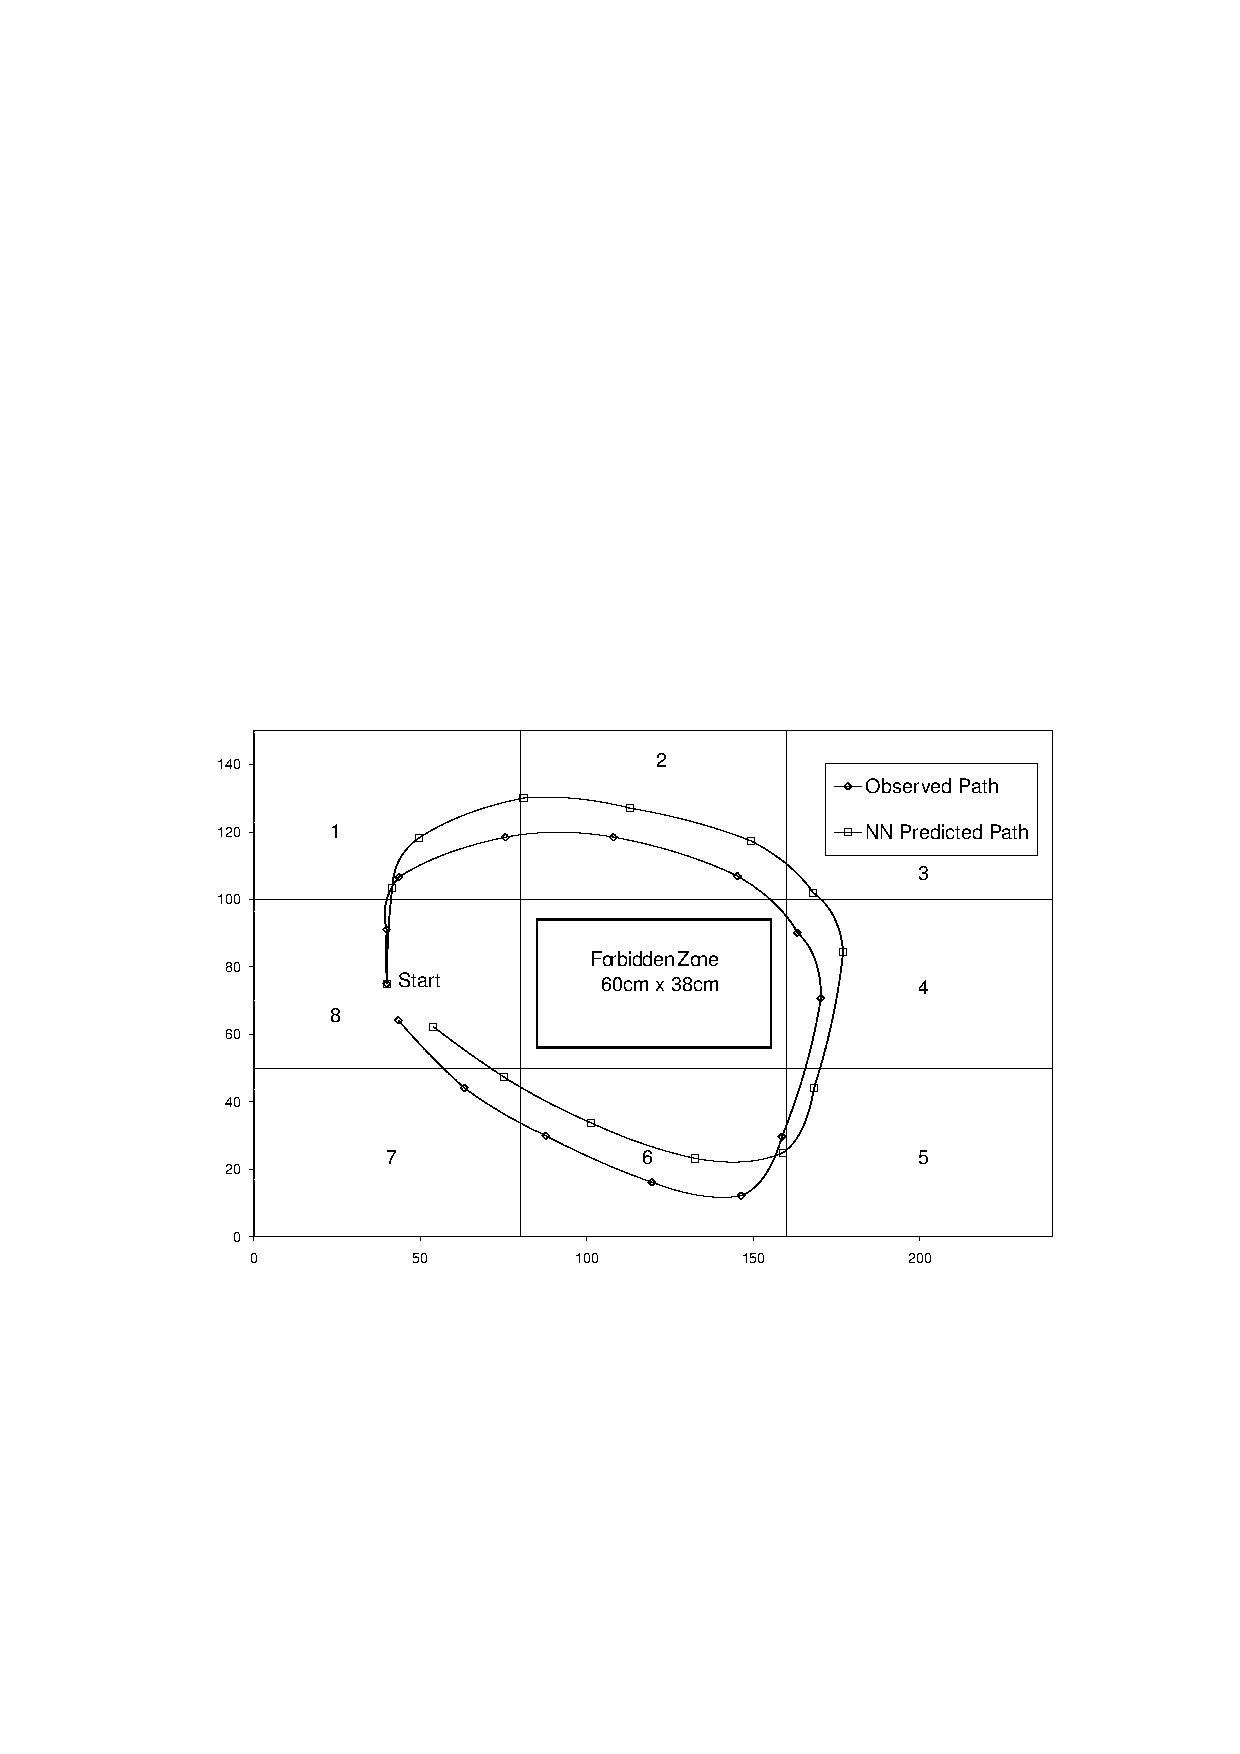
\includegraphics[scale=1]{cr3}
\label{fig:position tracking grid}
\end{figure*}
	  
\section{Conclusions}\label{conclusion}

 These research cases each demonstrate successful applications of ER. We can draw the conclusion that evolutionary robotics can be quite effective. Simulation provided an important platform upon which evolution could take place. That platform can be a physical representation of the robot and the environment, or by a sizable testbed as seen in the robot developed by Pretorius $et$ $al.$~\cite{Pretorius:2009:TAN:1632149.1632171}. Despite the problems presented by each of the research cases, each were able to find a suitable candidate solution, be it though ANN or parameter sets. Despite the diversity of environments and interactions robots may be subjected to, ER remains a useful tool.

 %The robots from the research cases tended to diversify when it came to observed behaviors. The station keeping robot developed by Moore $et$ $al.$ ~\cite{Moore:2013:ESK:2463372.2463402} evolved many interesting behaviors, however no single candidate was made to excel in all of the trials. This was because Moore $et$ $al.$ wanted the simulated robot to master a given trial to gain some understanding of what an effective action would be, and then encode that functionality on the robot. In contrast, the walking robot developed by Farchy $et$ $al.$ ~\cite{Farchy:2013:HRL:2484920.2484930} and the coordinate tracking robot by Pretorius $et$ $al.$ ~\cite{Pretorius:2009:TAN:1632149.1632171} directly used their candidate solution in the physical robot. 


%ACKNOWLEDGMENTS are optional
\section{Acknowledgments}


%
% The following two commands are all you need in the
% initial runs of your .tex file to
% produce the bibliography for the citations in your paper.
\bibliographystyle{abbrv}
\bibliography{AdrianBib}  % ElenaSample.bib is the name of the Bibliography in this case
% You must have a proper ".bib" file
%  and remember to run:
% latex bibtex latex latex
% to resolve all references
%
% ACM needs 'a single self-contained file'!
%
%APPENDICES are optional
%\balancecolumns

\end{document}

\appendix
%Appendix A
\section{Headings in Appendices}
The rules about hierarchical headings discussed above for
the body of the article are different in the appendices.
In the \textbf{appendix} environment, the command
\textbf{section} is used to
indicate the start of each Appendix, with alphabetic order
designation (i.e. the first is A, the second B, etc.) and
a title (if you include one).  So, if you need
hierarchical structure
\textit{within} an Appendix, start with \textbf{subsection} as the
highest level. Here is an outline of the body of this
document in Appendix-appropriate form:
\subsection{Introduction}
\subsection{The Body of the Paper}
\subsubsection{Type Changes and  Special Characters}
\subsubsection{Math Equations}
\paragraph{Inline (In-text) Equations}
\paragraph{Display Equations}
\subsubsection{Citations}
\subsubsection{Tables}
\subsubsection{Figures}
\subsubsection{Theorem-like Constructs}
\subsubsection*{A Caveat for the \TeX\ Expert}
\subsection{Conclusions}
\subsection{Acknowledgments}
\subsection{Additional Authors}
This section is inserted by \LaTeX; you do not insert it.
You just add the names and information in the
\texttt{{\char'134}additionalauthors} command at the start
of the document.
\subsection{References}
Generated by bibtex from your ~.bib file.  Run latex,
then bibtex, then latex twice (to resolve references)
to create the ~.bbl file.  Insert that ~.bbl file into
the .tex source file and comment out
the command \texttt{{\char'134}thebibliography}.
% This next section command marks the start of
% Appendix B, and does not continue the present hierarchy
\section{More Help for the Hardy}
The sig-alternate.cls file itself is chock-full of succinct
and helpful comments.  If you consider yourself a moderately
experienced to expert user of \LaTeX, you may find reading
it useful but please remember not to change it.
%\balancecolumns % GM June 2007
% That's all folks!
\end{document}